Here the protocol presented by Giordani et al. \cite{giordani2020} is summarised.
The aim of the protocol is to generate higher dimensional entanglement via the use of quantum walks.
The imagined setup of this protocol is that there are two labs, $A$ and $B$, which have a shared source of entangled qubits but are otherwise spatially separated and cannot interact with one another.

In this section the following notation is employed:
\begin{itemize}
    \item $\ket{\psi}_J$ is a state belonging to the subspace $\mathcal{H}_J = \mathcal{H}^{(A)}_J \otimes \mathcal{H}^{(B)}_J, J\in\{C,W\}$. It is a state that describes the combined state of the coins or walkers.
    \item $\ket{\psi}^{(K)}$ is a state belonging to the subspace $\mathcal{H}^{(K)} = \mathcal{H}^{(K)}_C \otimes \mathcal{H}^{(K)}_W, K\in\{A,B\}$. It is a state that describes the combined state of one of the quantum walks.
    \item  $\ket{\psi}^{(K)}_J$ is a state belonging to the subspace $\mathcal{H}^{(K)}_J$.
\end{itemize}

In this mathematical framework the overall Hilbert space comprises of two quantum walk subspaces,
\begin{align}
    \mathcal{H} &= \mathcal{H}^{(A)} \otimes \mathcal{H}^{(B)}\\
                &= \mathcal{H}^{(A)}_C \otimes \mathcal{H}^{(A)}_W \otimes \mathcal{H}^{(B)}_C \otimes \mathcal{H}^{(B)}_W.
\end{align}
Due to the difficulty in writing entangled states when the entangled spaces are not adjacent, the subspaces will instead be taken to be in the order
\begin{equation}
    \mathcal{H} = \mathcal{H}^{(A)}_W \otimes \mathcal{H}^{(B)}_W \otimes \mathcal{H}^{(A)}_C \otimes \mathcal{H}^{(B)}_C,
\end{equation} 
i.e. with the walker subspaces adjacent to each other and the coin subspaces adjacent to each other.

The basic premise of this protocol is this:
\begin{enumerate}
    \item Entangle the two coin spaces of the walkers $\mathcal{H}_C$ (figure \ref{fig:preparation}).
    \item Proceed with the quantum walk for some determined number of steps.
    \item Use a projective measurement $\mathcal{P}_\gamma = \ket{\gamma}\bra{\gamma}; \ket{\gamma}\in\mathcal{H}^{(A)}_C$ to then transfer the entanglement so that it solely exists in the subspace $\mathcal{H}^{(A)}_W \otimes \mathcal{H}^{(B)}_W \otimes \mathcal{H}^{(B)}_C$. $\ket{\gamma}$ can be defined by two complex parameters, $\theta$ and $\phi$ (see equation \ref{eqn:arb_qubit}), which therefore also define $\mathcal{P}_\gamma$.
    \item In similar fashion, find a projection $\mathcal{P}_\delta = \ket{\delta}\bra{\delta}; \ket{\delta}\in\mathcal{H}^{(B)}_C$ to transfer the entanglement to exist between the two walker subspaces, $\mathcal{H}_W$, only. $\ket{\delta}$ is defined in the same way as $\ket{\gamma}$.
    \item Accumulate entanglement in the walker subspaces by once more entangling the two coin spaces and repeating the protocol.
\end{enumerate}

\begin{figure}
    \centering
    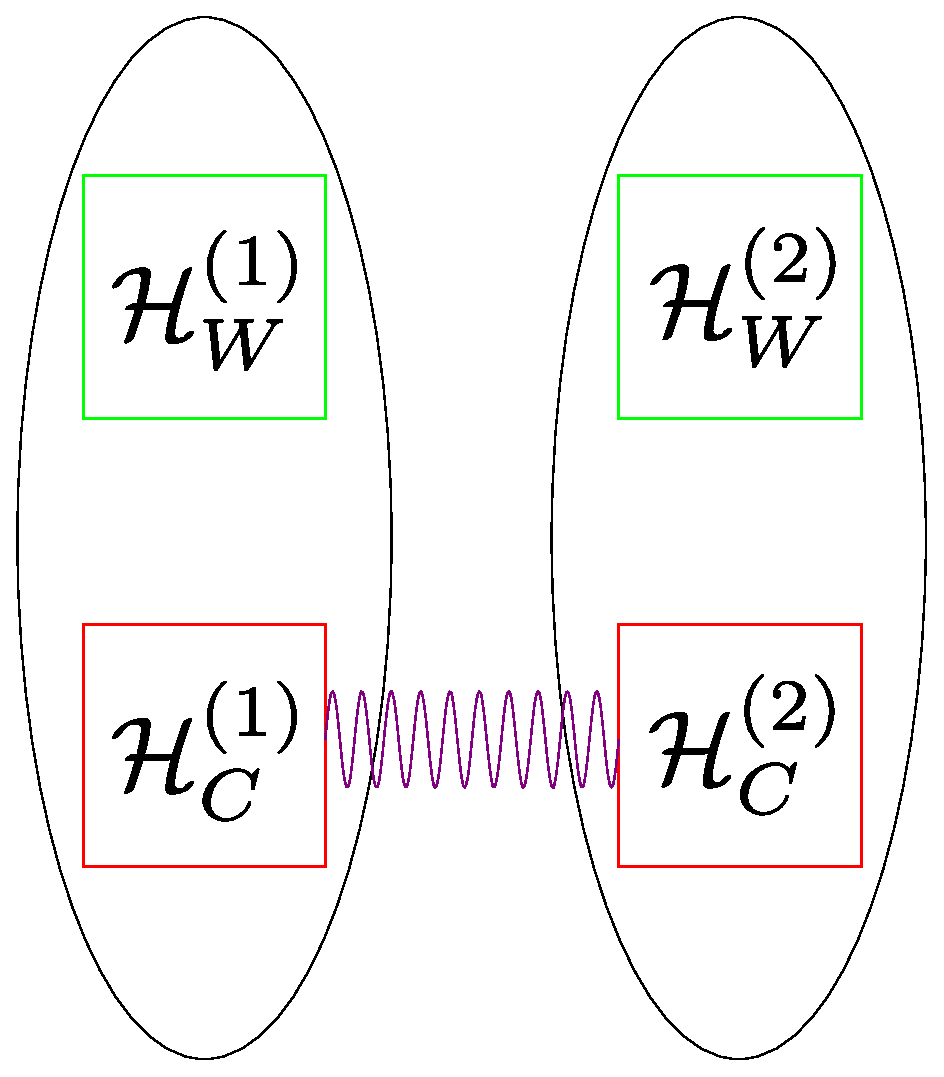
\includegraphics[scale = .25]{preparation}
    \caption{The initial prepared state has entanglement solely between the two coin subspaces. Figure is an edited version of FIG 3 from \cite{giordani2020}.}
    \label{fig:preparation}
\end{figure}
In this way, arbitrary amounts of higher dimensional entanglement can be generated.\newline
The ordering of steps 3 and 4 is not overly important since the full operators describing the projective measurements are given by
\begin{align}
    & I \otimes I \otimes \mathcal{P}_\gamma \otimes I \text{ and }\\
    &I \otimes I \otimes I \otimes \mathcal{P}_\delta,
\end{align}
which clearly commute.
As is the case with many quantum walk based protocols, particular attention must be paid to the choice of coin used for the quantum walk, as it will have a large impact on the success of the protocol.
The shift operator used to advance quantum walks is $\tilde{S}$, as outlined in section \ref{subsubsection:q_r_w}.
(More accurately it is $\tilde{S}^{(A)}\otimes\tilde{S}^{(B)}$, one for each walk, but for the sake of brevity $\tilde{S}$ will be used.)

\subsection{Transfer}
\label{subsection:qw_transfer}
To illustrate the basic principles of the protocol, consider the case where 
\begin{equation}
    C = I_d \otimes I_d \otimes \underbrace{I_2 \otimes I_2}_{\text{Coin operators}} = I.
\end{equation}
Note that this is not actually an instance of using quantum walk dynamics, since an identity coin equates to no coin at all.

\begin{enumerate}
    \item A state $\ket{\psi(0)}$ is prepared with the walkers at the origin and coin states entangled,
    \begin{equation}
        \ket{\psi(0)} = \ket{0}^{(A)}_W\ket{0}^{(B)}_W \otimes \underbrace{\frac{1}{\sqrt{2}}\Big [\ket{\uparrow}^{(A)}_C\ket{\uparrow}^{(B)}_C + \ket{\downarrow}^{(A)}_C\ket{\downarrow}^{(B)}_C \Big]}_{\text{Bell State}}.
    \end{equation}
    \item The "coin", $I$, is applied and followed by the shift operator $\tilde{S}$ to advance the quantum walks.
    Explicitly (dropping the indices and combining kets together) the two walks evolve to the state
    \begin{equation}
        \ket{\psi(1)} = \tilde{S}I\ket{\psi} = \frac{1}{\sqrt{2}}\Big [\ket{0,0}\ket{\uparrow,\uparrow} + \ket{1,1}\ket{\downarrow,\downarrow}\Big].
    \end{equation}
    Considering $\tilde{S}$ as $\C{X}$ then the control qubits are on the right and the target qudits are on the left here.
    \item Using the operator $\mathcal{P}_{\gamma} = \ket{\gamma}\bra{\gamma}$ the part of $\ket{\psi(1)}$ residing in the $\mathcal{H}^{(A)}_C$ subspace is projected onto the state $\ket{\gamma}$.
    
    For this example, choose $\ket{\gamma} = \frac{1}{\sqrt{2}} \big [\ket{\uparrow} + \ket{\downarrow} \big]$ which then gives
    \begin{equation}
        \mathcal{P}_\gamma \ket{\psi(1)} = \frac{1}{2}\Big [\ket{0, 0}\ket{\gamma,\uparrow} + \ket{1, 1}\ket{\gamma, \downarrow}\Big ].
    \end{equation}
    Here it is assumed that the projective measurement has given the correct state, but there is a 50\% chance that this projective measurement will project the coin onto $\ket{\gamma}^{\perp}$, the orthogonal state to $\ket{\gamma}$.
    It does not matter too much in this example if this happens, as the same amount of entanglement is transferred in either case.
    However this is not true in general, and post selection is needed to correct for this.

    \item Now, project the other coin onto $\ket{\delta}$ which in this instance is taken to be the same state, $\ket{\delta} = \frac{1}{\sqrt{2}} \big [\ket{\uparrow} + \ket{\downarrow} \big]$,
    \begin{equation}
        \mathcal{P}_\delta \mathcal{P}_\gamma \ket{\psi(1)} = \frac{1}{2}\Big [\frac{1}{\sqrt{2}}\Big (\ket{0, 0} + \ket{1, 1}\Big )\ket{\gamma}\ket{\delta}\Big].
    \end{equation}
    Again, it is assumed the projective measurement has given the correct state.
\end{enumerate}
Renormalising gives the final state
\begin{equation}
    \label{equation:qw_transfer_1_final}
    \underbrace{\frac{1}{\sqrt{2}}\Big [\ket{0, 0} + \ket{1, 1}\Big ]_W}_{\text{Bell State}}\otimes \ket{\gamma}^{(A)}_C \otimes \ket{\delta}^{(B)}_C,
\end{equation}
which has a Bell state in the $\mathcal{H}_W$ subspace, and the coin states are separable.
Therefore the entanglement that originally resided in the coin subspace has been transferred to the walker one.

\subsection{Accumulation}
\label{subsection:qw_accumulation}
The true motivation behind this protocol is the ability to accumulate the entanglement transferred from the lower dimensional coin subspace to the higher dimensional walker one.
This is done by repeating the entire process with some small changes.
Again $I$ is used as the coin operator and it is assumed the projective measurements succeed.
\begin{enumerate}

    \item Starting with the final state obtained from the first iteration of the protocol (equation \ref{equation:qw_transfer_1_final}), the coin subspaces are re-entangled, obtaining a new initial state $\ket{\psi(0)}$,
    \begin{alignat}{3}
        &&\frac{1}{\sqrt{2}}
        \Big [\ket{0, 0} + \ket{1, 1}\Big ]_W&\otimes \ket{\gamma}^{(A)}_C \otimes \ket{\delta}^{(B)}_C\\
        \overset{\text{Entangle coins}}{\longrightarrow}
        &&\frac{1}{2}\Big [\ket{0, 0} + \ket{1, 1}\Big ]_W &\otimes
        \Big [\ket{\uparrow, \uparrow} + \ket{\downarrow, \downarrow}\Big ]_C := \ket{\psi(0)}.
    \end{alignat}
    \item Now take two steps instead of one in the walk.
    \begin{align}
        \ket{\psi(2)} &= (\tilde{S}I)^2\ket{\psi(0)}\\
        &= \frac{1}{2}\Big[\big (\ket{0,0}+\ket{1,1}\big )\ket{\uparrow,\uparrow} + \big (\ket{2,2} + \ket{3,3}\big )\ket{\downarrow,\downarrow}\Big ].
    \end{align}
    \itemrange{1} Using the same projection operators in the two coin subspaces, $\mathcal{P}_\gamma \in \mathcal{H}^{(A)}_C,  \mathcal{P}_\delta \in \mathcal{H}^{(B)}_C$, and renormalising gives the final state
    \begin{equation}
        \frac{1}{2}\Big[\ket{0,0} + \ket{1,1} + \ket{2,2} + \ket{3,3}\Big ] \otimes \ket{\gamma}\otimes\ket{\delta}.
    \end{equation}
\end{enumerate}

Using claim \ref{claim:maximally_entangled_states}, the log negativity of
\begin{equation}
    \frac{1}{2}\Big[\ket{0,0} + \ket{1,1} + \ket{2,2} + \ket{3,3}\Big ]
\end{equation}
is 2, setting $d=4$ (since both of the walkers only have 4 states of non-zero amplitude they can be simulated by ququarts even if their true dimension is greater than 4).
Therefore, 2 units of log negativity have been transferred from the Bell states (each of log negativity 1) to the qudit pair and optimal transfer has been achieved.
The process can be repeated to accumulate arbitrarily large amounts of entanglement into our walker subspace.
The number of steps needed in the quantum walk for each iteration is as follows.
\begin{claim}
\label{claim:min_steps}
The $n^{\text{th}}$ iteration (counting from 1) of the protocol requires $2^{n-1}$ steps in the quantum walk.
\end{claim}
A proof of this is given in appendix \ref{appendix:min_steps}.

\subsection{Retrieval}
\label{subsection:qw_retrieval}
Although accumulating the entanglement in higher dimensions is of significant use, it is also possible to imagine that retrieving the entanglement back into the qubits would also be of interest.
For example, consider the case where the method of generating entangled qubits is not deterministic, or takes a reasonably long time, but an algorithm requiring large numbers of Bell states is to be executed.
If the accumulation of entanglement can be reversed to get Bell pairs back, then the entangled Bell pairs can be stored in the qudits when they are successfully generated and then retrieved all at once to ensure the algorithm can be performed.
In principle, it is possible to use a similar quantum walk setup where the entangled qudits are the coins and the qubits are the walkers to get entanglement back out.
However due to the non-unitary nature of the protocol (the projective measurements are irreversible), this setup is not simple to design.

\subsection{Results}
\label{subsection:results}
Despite its simple construction, the state of a quantum walk becomes extremely complex after even just a few steps in most cases.
This is doubly true for two quantum walks running in conjunction.
Hence, numerical simulations were employed to analyse the protocol in settings that are not as trivial as the identity coin example.
When transferring entanglement from only one Bell pair, the protocol was able to use Hadamard-coined quantum walks to optimally transfer the entanglement to the qudits (this is shown in appendix \ref{appendix:qw_figures} figure \ref{fig:1ebit_transfer}).
When simulating the accumulation of two and three Bell pairs of entanglement, again using Hadamard-coined QWs, figure \ref{fig:lneg_transfer} shows that the protocol can generate states with log negativities of up to approximately 1.585 and 2.036 respectively if using the same $\mathcal{P}_\gamma$ for both coins.
Simulations were also done using different projective operators $\mathcal{P}_\gamma$, $\mathcal{P}_\delta$ to transfer entanglement from two Bell states.
These also showed $\sim 1.585$ is still the maximum possible when using the Hadamard coin.
Sample plots from simulations with differing projective operators are found in appendix \ref{appendix:qw_figures} figure \ref{fig:2ebits_diff_proj}.

The relationship between the bias of a coin with real coefficients (equation \ref{eqn:general_coin}) and the maximum log negativity of the combined walker state is plotted in figure \ref{fig:bias_lneg}.
It highlights how entanglement transfer gets closer to being optimal as the coin gets closer to the identity, at which point there are no quantum walk dynamics at all - the protocol works better the less it resembles a quantum walk.

Furthermore, all of this analysis is done with the assumption that the projective measurements succeed.
This is not true in general and the procedure has to be repeated if the projective measurements project onto the orthogonal states.
For example, an experimental proposal using photons as both the coins and walkers is given in \cite{giordani2020} which requires post-selection, where the final state of the walkers is discarded if the projective measurements result in undesired states.

In light of this, it is fair to conclude that the choice to facilitate entanglement transfer via quantum walks is an impractical one.
However, given that the protocol has the potential to work optimally, it is worth reconstructing it in an alternative model of quantum computing, whose constraints can lead to optimal transfer being the natural outcome of the model.
\begin{figure}[h]
    \centering
    \begin{subfigure}{0.49\textwidth}
        \centering
        $E_\mathcal{N}$\\
        \includegraphics[width = \linewidth]{2ebit_transfer.png}
        \caption{Transferring entanglement from two Bell states. Red points correspond to $E_\mathcal{N}\sim 1.585$.}
        \label{fig:2ebittransfer}
    \end{subfigure}
    \hfill
    \begin{subfigure}{0.49\textwidth}
        \centering
        $E_\mathcal{N}$\\
        \includegraphics[width = \linewidth]{3ebittransfer.png}
        \caption{Transferring entanglement from three Bell states. Red points correspond to $E_\mathcal{N}\sim 2.036$.}
        \label{fig:3ebittransfer}
    \end{subfigure}
    \caption{Log negativity, $E_\mathcal{N}$, of combined walker states using the QW transfer protocol. $\theta, \phi$ are the parameters defining $\mathcal{P}_\gamma,\mathcal{P}_\delta$ where $\mathcal{P}_\gamma = \mathcal{P}_\delta$ for both simulations. Both walks were conducted using the Hadamard coin. Red points indicate peak values of log negativity on the plots. $\theta$ and $\phi$ are each varied over 100 evenly spaced values.}
    \label{fig:lneg_transfer}
\end{figure}

\begin{figure}[h!]
    \centering
    \includegraphics[width = 0.55\textwidth]{bias_max_lneg.png}
    \caption{Peak $E_\mathcal{N}$ of walkers after transferring entanglement from two Bell pairs using quantum walks with coins of varying bias, $\rho$. The peak value was found by computing the largest value of log negativity for 100 evenly spaced values of both $\theta$ and $\phi$, the parameters for the coin projection operators $\mathcal{P}_{\gamma}, \mathcal{P}_\delta$ where $\mathcal{P}_{\gamma} = \mathcal{P}_\delta$.}
    \label{fig:bias_lneg}
\end{figure}